\chapter{Fallstudien}\label{scenarios}
\begin{comment}
subsection{Fallstudie Rossi Notes}

Fragestellungen:
Wie kann das 3D Modell eines Gebäudes zu einem für einen Roboterschwarm abarbeitbaren Bauplan umgewandelt werden?
Folgefragen:
Wie werden Gebäude heutzutage modelliert? (Revit, Blender -> IFC BIM)
Wie sieht das Format des 3D Modells aus? (IFC)
Was sind gägnige Praktiken beim Planen eines Bauprojekts? (BIM)
Wie ist der aktuelle Stand der Automatisierung im Bereich Konstruktion? (Related Work)
Welche Projekte bauen schon mit Roboter(schwärmen) Gebäude/Gebilde? (Related Work)
Welche Schwierigkeiten gibt es? (Related Work)
Wie sieht so ein Bauplan aus? (Ludwigs Diss)
Welche Schwierigkeiten gibt es bei der Erstellung so eines Bauplans?  (Ludwigs Diss)

Fallstudie:
Modellieren eines Gebäudes in einem 3D Editor, welches anschließend in einen Bauplan überführt wird.

Suche:
3D Editor.
Speicherformat für 3D Modelle.

Probleme: 
Analaysie des 3D Modells auf für uns notwendige Teile (Wände zb)
Mit einbeziehen sämtlicher Constraints von Robotern und Bauteilen (Form Bewegungseinschränkungen Stapelbarkeit etc).
Für Roboter erstmal nicht überbrückbare Lücken wie Fenster Türen.
Guten/Besten Bauplan generieren (Ludiwgs Diss).

Heterogener Roboterschwarm baut Haus mit Fenstern und Türen (Lücken)
Wie werden arbiträre Bausteine beschrieben, damit damit dann ne Wand gefüllt werden kann. Kann man die Bausteine schneiden und wenn ja wo und welcher Weise?


\begin{figure}
    \centering
    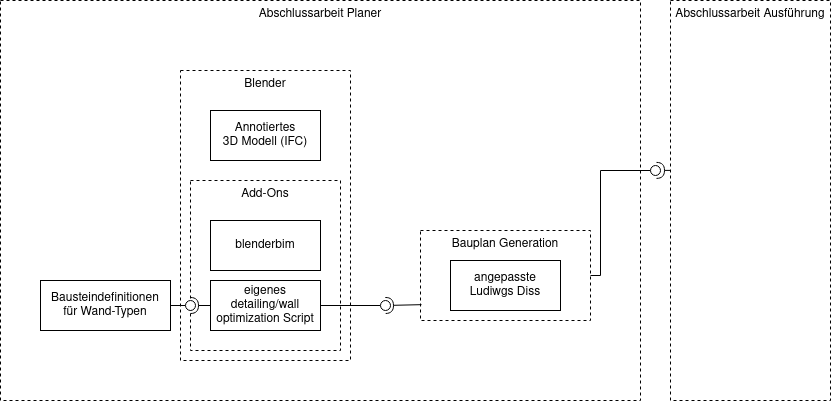
\includegraphics[width=0.9\columnwidth]{fig/structure.drawio.png}
    \caption{Aufbau der Abschlussarbeiten}
    \label{fig:Structure}
\end{figure}

Die Fallstudie unterteilt sich in zwei Teile, die jeweils von einer selbständigen Abschlussarbeit bearbeitet werden.
Der vorliegende erste Teil behinhaltet das Modellieren eines Gebäudes in einem 3D Editor und das anschließende Analysieren und Errechnen eines Bauplans.
Der Bauplan soll im zweiten Teil der Fallstudie von speziell dafür entwickelten Robotern durchgeführt werden, die sich auf den Mauern des Gebäudes selbst bewegen.
Dabei soll das Gebäude Elemente wie Fenster und Türen enthalten, um dem Problem von Lücken innerhalb einer Wand zu begegnen, welche ein Hindernis für die darauf fahrenden Roboter darstellen.
Das Errechnen eines Bauplans ausgehend von einem 3D Modell eines Gebäudes soll für beliebig beschaffene Bausteine möglich sein, welche zuvor definiert werden.
\end{comment}

\section{Planung und Bauplandeduktion eines LEGO Gebäudes mit Einsteinmauerwerk}
Ziel dieses Szenarios ist es, aus dem in Abbildung \ref{fig:Scenario1 Screenshot} dargestellten 3D Modell ein Bauplan zu generieren.
\begin{figure}[ht]
  \begin{subfigure}[b]{0.44\columnwidth}
    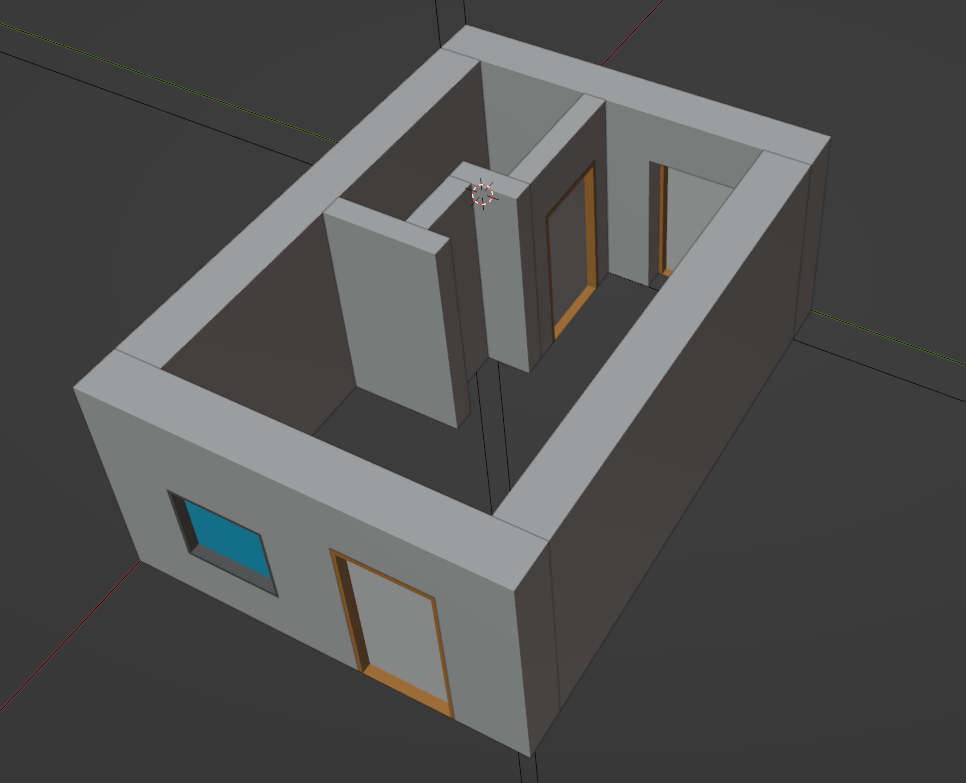
\includegraphics[width=\columnwidth]{fig/scenario1_screenshot.png}
    \caption{3D Modell innerhalb von Blender.}
    \label{fig:Scenario1 Screenshot}
  \end{subfigure}
  \hfill
  \begin{subfigure}[b]{0.505\columnwidth}
    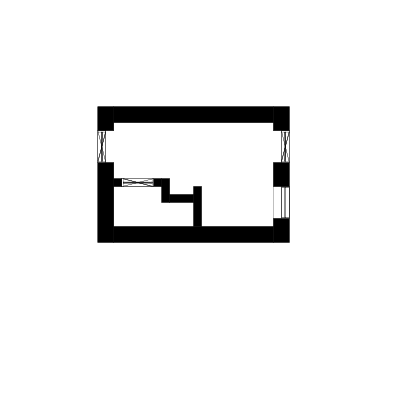
\includegraphics[width=\columnwidth]{fig/scenario1_story_plan.jpg}
    \caption{Gebäudeplan des 3D Modells.}
    \label{fig:Scenario1 Gebäudeplan}
  \end{subfigure}
  \label{fig:Scenario1 komplett}
  \caption{Modell eines Studentenzimmers (verschiedene Darstellungsformen).}
\end{figure}
Zu sehen ist der Plan eines einfachen Hauses mit einem Stockwerk.
Dieses besitzt eine Eingangstür, eine Terassentür neben einem Fenster und eine Tür, die das Badezimmer vom Hauptraum trennt.
Türen und Fenster stellen eine Herausforderung für den Planungsalgorithmus dar, da der Verlauf einer ansonsten durchgängigen Wand dadurch unterbrochen wird und Lücken aufweist.
Details wie Duschen, Betten, Toiletten und ähnliche Komponenten, sind für dieses Szenario irrelevant, da diese keinen Effekt auf die Struktur der Wände haben und wurden aus diesem Grund bewusst weggelassen.
Das Modell wurde mithilfe der in Kapitel \ref{basics} näher behandelten Technologien erstellt und enstpricht in seiner Struktur einem verbreiteten Industriestandard.
Dafür wurden zwei Wandtypen definiert, die jeweils unterschiedliche Wanddicken vorgeben.
So gibt es breite Außen- und dünne Innenwände.
Diese entsprechen in ihren Maßen dem Raster, welches das \textit{LEGO System} (siehe Kapitel \ref{basics}) vorgibt.
Für breite Wände gilt, dass diese immer zwei Noppen breit, mindestens eine Noppe lang und einen Stein hoch sein muss.
Für dünne Wände hingegen gilt eine feste Breite von einer Noppe, ebenfalls eine Mindestlänge von einer Noppe und eine Mindesthöhe von einem Stein.
Beide Wandtypen können nur Höhen beziehungsweise Längen aufweisen, die jeweils einem Vielfachen der Höhe oder Länge des kleinsten Legosteins aufweisen, der zum Bau der Wände verwendet werden soll (hier der 1x1 Stein).
Daraus resultiert ein Raster, welches ebenfalls für die Ausmaße und Positionen der Fenster und Türen einzuhalten ist.
Dieses Raster gilt es, abhängig des ausgewählten Wandtyps, in den Editor zu integrieren, um das Modellieren solcher Gebäude nutzerfreundlich zu gestalten und nicht durch ständiges Messen und Eintragen genauer Positionen oder Maße zu unterbrechen.
\begin{figure}[!ht]
    \centering
    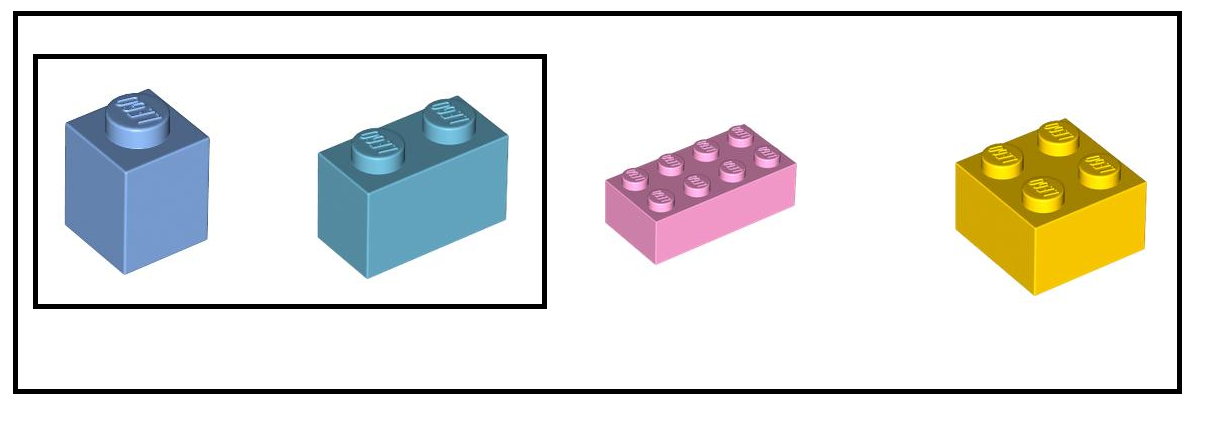
\includegraphics[width=0.6\columnwidth]{fig/scenario1_lego_set.png}
    \caption{LEGO Steintypen für die Innen- und Außenwände. (TODO Bild ist sehr hässlich)}
    \label{fig:Scenario1 Lego Set}
\end{figure}
Nicht nur die Abmessungen der Wände müssen in ein Raster fallen, auch deren Rotation wird in diesem Szenario auf 90\textdegree{} Schritte limitiert. 
Das stellt in diesem Fall eine vertretbare Enschränkung dar, da es ohnehin dem intuitiven Umgang mit LEGO Steinen und gleichzeitig dem Baustil der meisten einfachen Gebäuden entspricht.
Folglich muss ein Format für die Bausteintypen entwickelt werden, aus welchen all diese Informationen abgeleitet werden können.
Dieses Format muss sowohl von dem Editor selbst verwendet, als auch zur Berechnung innerhalb des Planungsalgorithmus herangezogen werden.
Außerdem werden weitere Regeln benötigt, um den resultierenden Plan näher an das Vorgehen eines realen Baus zu bringen.
So werden beim Errichten von Häusern zuerst die Ecken (der Schnittpunkt zweier Wände) um eine Stufe erhöht, um im Anschluss die geraden Wandabschnitte aufzufüllen.
Damit wird vermieden, dass in den ohnehin schon komplexeren Eckbereichen auch noch zugeschnittene Ziegel notwenig werden.
Stattdessen schneidet man diese erst zurecht, wenn sich dann eher mittig im Wandabschnitt Lücken ergeben, die kleiner sind als die vorhandenen Ziegel.
Zwar wird dies im Fall von Legosteinen nie auftreten, aber es ist übersichtlicher das Problem in dem vorliegenden eingeschränkten Szenario zu beschreiben.
Zusätzlich müssen Regeln in den Planungsalgorithmus eingeführt werden, die diverse Mauerwerksverbände (vorgestellt in Kapitel \ref{basics}) erzwingen zu können, um damit die Stabilität und gleichmäßige Kraftverteilung innerhalb einer Wand zu gewährleisten und sich ebenfalls möglichst nah an der Realität des Mauerbaus zu bewegen.

Einschränkungen:
 * Alle Wände verwenden ein Ziegelset, in welchem alle Ziegel die gleiche Höhe haben
 * Alle Wände verwenden den selben Mauerwerksverband
 * Alle anderen sich berührenden Wäände stehen in einem 90 Grad Winkel zueinander

\subsection{Problemstellung}
\label{scenarios:scenario1:problem}
Bevor für das Modell ein passender Bauplan entwickelt werden kann, muss das sogenannte \textit{Wall Detailing} (vgl. Kapitel \ref{basics:wall-detailing}) stattfinden.
Darunter versteht man das Berechnen einer Bausteinkombination, die eine Wand möglichst gut abbildet.
Dabei bedeutet "möglichst gut", dass die Proportionen der Bausteinkombination möglichst den der Ursprungswand entsprechen und keine nicht gewollten Lücken entstehen.
In diesem Szenario wird durch Auflegen des Rasters des LEGO Systems schon während des Modelliervorgangs sichergestellt, dass das resultierende Modell mit Legosteinen baubar ist.
Darum ist das Ziel des \textit{Wall Detailing} Schrittes in diesem Szenario, jede Wand lückenlos mit Bausteinen zu füllen.
Zusätzlich existieren folgende Einschränkungen und Eigenschaften, die für das Ergebnis dieses Szenarios gelten sollen.

\paragraph{Überbindemaß}
Obwohl in dem vorliegenden Modell ausschließlich Einsteinmauerwerke vorgesehen sind, gilt es die in Kapitel \ref{basics:Mauerwerksverband} erläuterte Regel zum Überbindemaß von Bausteinen zu beachten.
Da es sich hierbei aber um LEGO Steine handelt, die wesentlich kleiner sind als die genormten Formate für Ziegelsteine, wird der für das Überbeindemaß vorgesehene Mindestwert von 45mm ignoriert.
Außerdem ist ein Versatz von unter 50\% der Dicke eines Legosteines in den meisten Fällen nicht umsetzbar, da diese nicht frei übereinander gesteckt werden können.
Darum wird für dieses Szenario wird ein Überbindemaß von exakt 50\% der Steindicke verwendet, was den Einschränkungen des Überbindemaßes entspricht, welches einen Mindestversatz von 40\% der Steindicke voraussetzt.
Für die in Abbildung \ref{fig:Scenario1 Lego Set} dargestellten Lego Steine kann mit einem solchen Überbindemaß gleichzeitig auch das vorgesehene Raster des Lego Systems eingehalten werden, da diese alle eine gerade Anzahl an Noppen besitzen.
TODO Bild von dumm gestapelter LEGO Wand zu LEGO Wand mit Überbindemaß.

\paragraph{Anstoßende Wandstücke} 
Besonders herausfordernd ist die Einhaltung des Überbindemaßes an anstoßenden Wandstücken.
Solche Wandstücke entstehen zum Beispiel an Ecken, also 90 Grad zueinanderstehende Wände oder aber an den Übergängen von Außenwänden zu Innenwänden.
Wie in Abbildung \ref{fig:Scenario1 Screenshot} zu erkennen treten in diesem Szenario beide Fälle auf.
Zunächst müssen daher alle anstoßenden Wandstücke aus dem Modell gefiltert werden.
In Kapitel \ref{basics:Mauerwerksverband} werden gängige Praktiken zur Lösung von anstoßenden Wandstücken vorgestellt.
Mit diesen Informationen muss der Planungsalgorithmus zunächst eine Lösung für solche Wandstücke finden und anschließend die restlichen Flächen mit dem Vorgehen von oben auffüllen.

\paragraph{Öffnungen}
Das Fenster und die drei Türen sind hier die einzigen Besonderheiten in dem Modell.
Für den Mauerbau bedeutet dies an den entsprechenden Stellen Öffnungen zu lassen.
Die Informationen über diese Öffunungen liegen innerhalb des Formates vor, in welchem das Modell erstellt wurde (siehe \ref{basic:IfcOpeningElement}).
So lassen sich Größe und Position leicht herausfinden und das Ergebnis der beiden obigen Schritte dementsprechend abändern.

Nun liegt eine Beschreibung des Modells mit dem zuvor definierten Set an Legosteinen vor.
Als letzten Schritt gilt es daraus eine Abfolge an Bauinstruktionen zu finden, die unter Beachtung von diversen Einschränkungen zum gewünschten Ergebnis führen.
Mit dieser Problemstellung hat sich Ludwig (TODO) in  seiner Dissertation auseinandergesetzt (siehe Kapitel \ref{related:ludwigs dis}). 
Einschränkungen, die beim Bau von Legokonstruktionen gelten sind:
Deadlock, Überhang etc. (TODO)
Das Vorgehen in seiner Arbeit soll für dieses Szenario evaluiert und gegebenenfalls angepasst werden.


\section{Planung und Bauplandeduktion eines Lego Gebäudes mit Verbandsmauerwerk}
Kein Einsteinmauerwerk -> dicke Wände, die mit Läufern und Bindern erstellt werden müssen.
Eckfälle sehr komplex (siehe Basics)

\section{Szenario mit veränderbaren Bausteintypen}
Wie können wir die Bausteine veränderbar machen, sprich die Bearbeitungsmöglichkeiten während des Baus (schneiden eines Ziegels) miteinbeziehen in unser Bausteinformat.
Erstmal das schneiden nur parallel zu den ebenen eines rechteckigen ziegelsteins betrachten, denn bei "schrägen" schnitten entstehen neue komplexe Formen..
Wie generiert man daraus dann Baupläne -> riesiges aber cooles Optimierungsproblem!
Vlt geht das richtung constraint programming? Sprich den Bauplan als Lösung für ein beschränktes Problem ansehen.
Total viele Fragen, keine Ahnung wo zu beginnen aber klingt cool

\section{Sternchenaufgabe: Szenario mit "runden" Wänden und arbiträren (nicht rechteckige) Bausteinformen / schräge schnitte}
Was machen wir wenn die Wand nicht perfekt mit den vorgegebenen Bausteintypen gebaut werden kann (Beispiel ein runder Turm)
Bausteinverbindungen (wie Mörtel) betrachten und als \textit{Verbindungselement} in das Bausteinformat mit aufnehmen? Wie kann man diesen so einschränken, dass nur physisch machbares ausgrechnet wird.
Was wenn die Bausteine arbiträre Formen haben und nur in sehr komplexen Mustern eine "dichte" Wand ergeben -> tiling Probleme.